\chapter{Estado de la Cuestión Concursos de Programación}

\label{cap:concursos_programacion}

\chapterquote{Asturias es el único lugar del mundo donde la lluvia no entristece, sino que limpia el alma y enciende el paisaje}{Azorín}

\section{Concursos de Programación}
\label{sec:concursos_programacion}

Un concurso de programación es una competición en la que equipos de participantes deben resolver un conjunto de problemas algorítmicos en un tiempo limitado, generalmente entre tres y cinco horas. El formato más extendido en el ámbito universitario es el estilo ICPC (\textit{International Collegiate Programming Contest}), donde grupos de tres estudiantes compiten de forma simultánea enviando soluciones a un sistema de jurado automático que las evalúa en tiempo real \citep{DOMjudge}. El ganador es el equipo que resuelve más problemas correctamente, con el tiempo total acumulado como criterio de desempate en caso de igualdad.

Durante el concurso, el \textbf{marcador} (\textit{scoreboard}) recoge en todo momento la clasificación de los equipos, el número de problemas resueltos, los intentos fallidos y el tiempo empleado. Este marcador es público y se actualiza en tiempo real, lo que convierte su retransmisión en un elemento central de la experiencia del espectador. Además, cada envío de código genera un \textbf{evento} que puede visualizarse al instante: el equipo que ha enviado, el problema intentado y el veredicto obtenido (\textit{Accepted}, \textit{Wrong Answer}, \textit{Time Limit Exceeded}, entre otros). La figura~\ref{fig:juez1} muestra el aspecto del sistema de jurado durante un concurso en curso.

\begin{figure}[H]
  \centering
  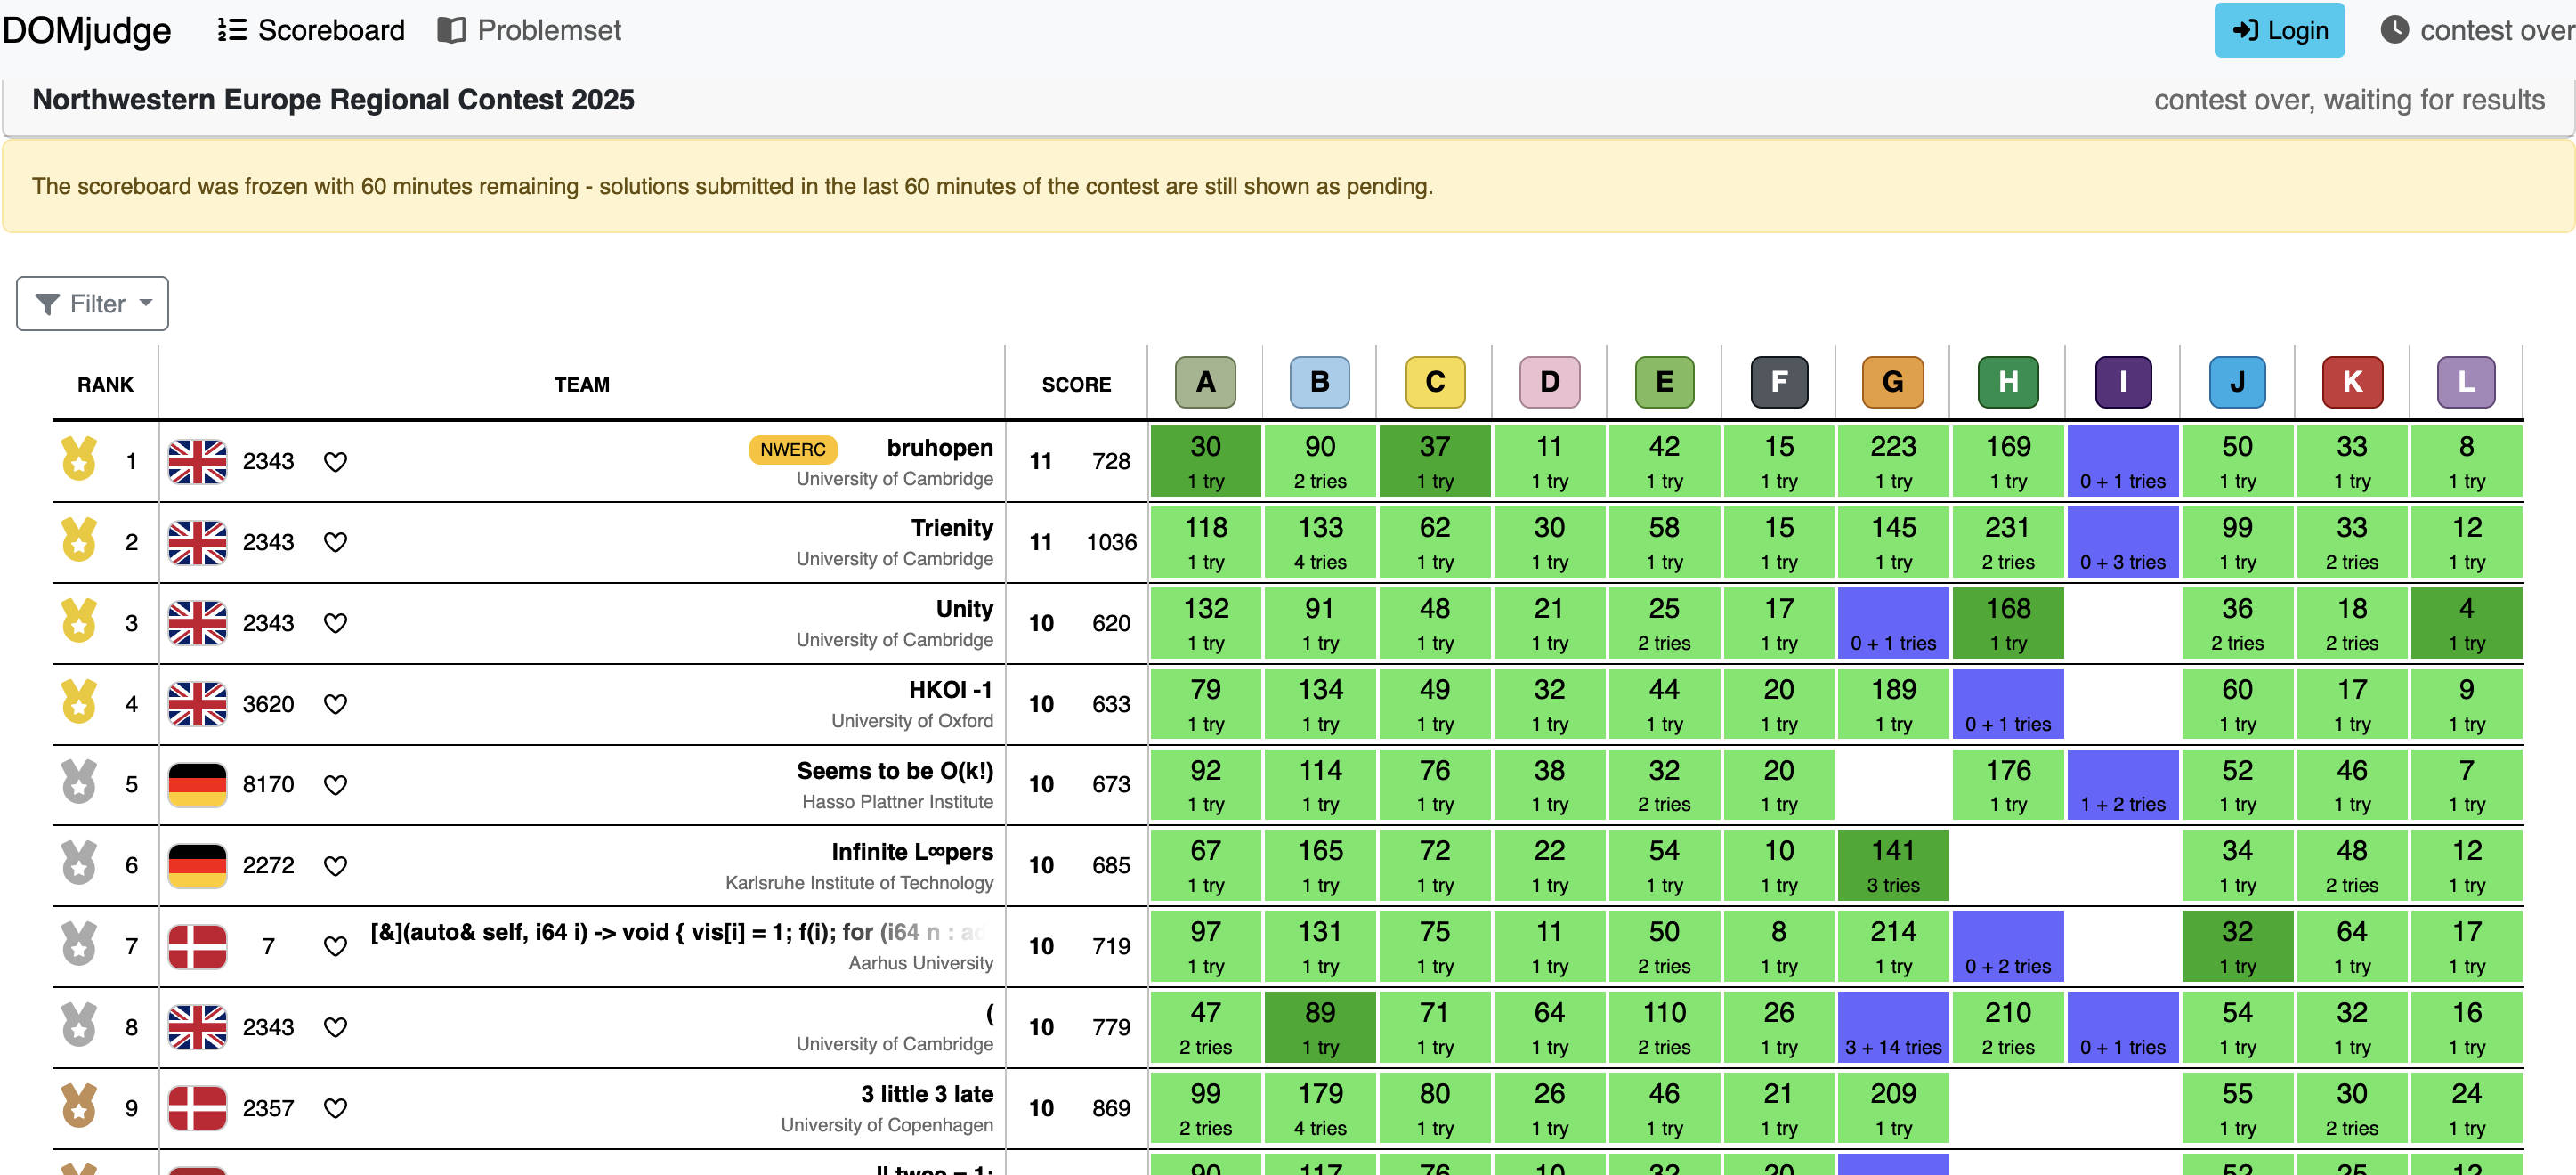
\includegraphics[width=\textwidth]{Imagenes/Vectorial/juez1.png}
  \caption{Vista del sistema de jurado automático durante un concurso de programación, mostrando los equipos participantes y el estado de sus envíos en tiempo real.}
  \label{fig:juez1}
\end{figure}

\subsection{Objetivos de los concursos de programación}

Los concursos de programación tienen un doble propósito. Por un lado, constituyen una herramienta pedagógica de gran valor: enfrentarse a problemas inéditos con restricciones estrictas de tiempo y recursos obliga a los participantes a desarrollar pensamiento algorítmico, capacidad de abstracción y habilidad para identificar rápidamente qué estructura de datos o estrategia de resolución es la adecuada en cada situación. Competir en equipo con un único ordenador fuerza además la comunicación, la división del trabajo y la gestión del tiempo bajo presión, habilidades directamente transferibles al entorno profesional del desarrollo de software.

Por otro lado, los concursos son una plataforma de excelencia competitiva reconocida internacionalmente. El circuito ICPC, con presencia en más de cien países y miles de universidades, culmina cada año en unas Finales Mundiales donde los mejores equipos del planeta se enfrentan a problemas que, en ocasiones, no son solucionados por ningún equipo durante el tiempo del concurso. Esta dimensión ha convertido a los concursos de programación en un referente del sector tecnológico: grandes empresas como Google, Meta y Amazon patrocinan activamente el ICPC y utilizan los resultados como indicador de talento técnico excepcional.

En el contexto universitario español, la competición más representativa es el Ada-Byron, organizado por la asociación SEDI, que sigue el formato ICPC. Los equipos clasificados en las fases regionales acceden a la final nacional, y desde ahí los mejores pueden representar a España en las finales europeas y mundiales. Este ecosistema hace que los concursos sean eventos de relevancia académica con una audiencia de participantes, jueces, profesores y espectadores que demanda retransmisiones de calidad.

\subsection{Formato ICPC y dinámica del concurso}

El formato ICPC establece reglas muy precisas que condicionan los requisitos del sistema de jurado y la dinámica del evento.

Cada \textbf{equipo} está formado por exactamente tres estudiantes que comparten un único ordenador durante toda la competición. Esta restricción de hardware no es accidental: obliga al equipo a organizarse, trabajar en papel o pizarra mientras un miembro escribe en el ordenador, y consensuar decisiones sobre qué problema abordar en cada momento. La duración estándar es de \textbf{cinco horas}, durante las cuales los equipos pueden leer y resolver los problemas en cualquier orden.

El conjunto de problemas, llamado \textit{problem set}, consta habitualmente de entre diez y trece enunciados de dificultad heterogénea. Cada problema requiere que el equipo programe una solución que lea datos de la entrada estándar y escriba el resultado en la salida estándar, dentro de los límites de tiempo y memoria establecidos. Las soluciones se envían en el lenguaje elegido por el equipo (habitualmente C, C++ o Java) y son evaluadas automáticamente contra un conjunto de casos de prueba no visibles para los participantes.

El \textbf{sistema de globos} es uno de los elementos más visuales del formato ICPC: cuando un equipo resuelve un problema por primera vez, un voluntario acude a su puesto con un globo del color asignado a ese problema. Los globos en cada puesto indican de un vistazo qué problemas ha resuelto cada equipo, creando un elemento visual inmediato tanto para los participantes como para el público y los retransmisores.

La \textbf{penalización por envíos incorrectos} es otro mecanismo clave: cada envío fallido a un problema que el equipo termina resolviendo suma veinte minutos al tiempo total de penalización. Esto desincentiva los envíos irreflexivos y hace que la estrategia, cuándo enviar y cuándo depurar más antes de hacerlo, sea parte del juego competitivo. Dos equipos con el mismo número de problemas resueltos quedan ordenados por tiempo total de penalización, lo que significa que la diferencia puede ser de un solo minuto.

El \textbf{congelamiento del marcador} (\textit{scoreboard freeze}) es la característica más dramática del formato ICPC: durante la última hora del concurso, el marcador deja de actualizarse públicamente. Los envíos recibidos en ese período son juzgados con normalidad, pero sus resultados son invisibles para el público y para los demás equipos. Esto genera una tensión notable porque la clasificación final puede diferir radicalmente de la que se mostraba antes del congelamiento. Esa diferencia se desvela en la ceremonia de clausura mediante la \textbf{resolución del marcador} (\textit{scoreboard reveal}), donde los resultados se muestran problema a problema, de atrás hacia adelante, con la emoción creciente de cada cambio de posición. Este momento es precisamente el que una retransmisión enriquecida con RA puede hacer más espectacular.

\subsection{Veredictos del juez automático}

Cada envío recibe un veredicto del sistema de jurado. Los más habituales en el estilo ICPC son los siguientes:

\begin{itemize}
  \item \textbf{Accepted (AC):} la solución produce la salida correcta en todos los casos de prueba dentro de los límites establecidos. El problema queda marcado como resuelto.
  \item \textbf{Wrong Answer (WA):} la salida es incorrecta en al menos un caso de prueba. Añade penalización si el equipo acaba resolviendo el problema.
  \item \textbf{Time Limit Exceeded (TLE):} la solución no termina dentro del tiempo máximo permitido para el problema. Indica un algoritmo con complejidad computacional demasiado elevada.
  \item \textbf{Memory Limit Exceeded (MLE):} la solución supera el límite de memoria permitido.
  \item \textbf{Runtime Error (RE):} la solución produce un error en tiempo de ejecución (segmentation fault, excepción no capturada, etc.).
  \item \textbf{Compilation Error (CE):} el código no compila. Generalmente no añade penalización.
  \item \textbf{Pending (PEND):} el envío ha sido recibido pero aún no ha sido juzgado, relevante especialmente durante el congelamiento.
\end{itemize}

Estos veredictos son los que el sistema de jurado automático comunica a través de su API, y son la base sobre la que el plugin de RA construye la visualización de eventos: cada veredicto \textit{Accepted} es un evento que puede mostrarse en pantalla con el nombre del equipo, el problema resuelto y su nueva posición en el marcador.

\subsection{Infraestructura tecnológica: el CMS}

La infraestructura tecnológica que soporta estos eventos recibe el nombre de \textit{Contest Management System} (CMS). El CMS se encarga de recibir los envíos, compilarlos y ejecutarlos en un entorno aislado, publicar el marcador actualizado y notificar el veredicto de forma inmediata. En la siguiente sección se describe el CMS empleado en este trabajo: DOMjudge.

\section{DOMjudge}
\label{sec:domjudge}

DOMjudge \citep{DOMjudge} es el sistema de gestión de concursos de referencia en el ámbito universitario y competitivo. Se trata de una aplicación web de código abierto desarrollada de forma colaborativa por la comunidad, adoptada como sistema oficial de la ICPC a nivel mundial y empleada en numerosos eventos regionales y nacionales, incluidos los concursos universitarios en España.

\subsection{Arquitectura}

Su arquitectura separa dos componentes claramente diferenciados. El \textit{DOMserver} actúa como servidor central: gestiona la base de datos del concurso, sirve la interfaz web a participantes, jueces y administradores, y expone una \textbf{API REST} para la integración con sistemas externos. Los \textit{judgehosts} son los nodos encargados de compilar y ejecutar el código enviado por los participantes en un entorno aislado y seguro, generalmente mediante \textit{cgroups}. Esta separación permite escalar el sistema añadiendo judgehosts sin modificar el servidor central: en concursos con muchos participantes simultáneos se pueden desplegar varios judgehosts en paralelo para reducir los tiempos de espera. La figura~\ref{fig:juez2} muestra la interfaz de administración de DOMjudge durante un concurso.

\begin{figure}[H]
  \centering
  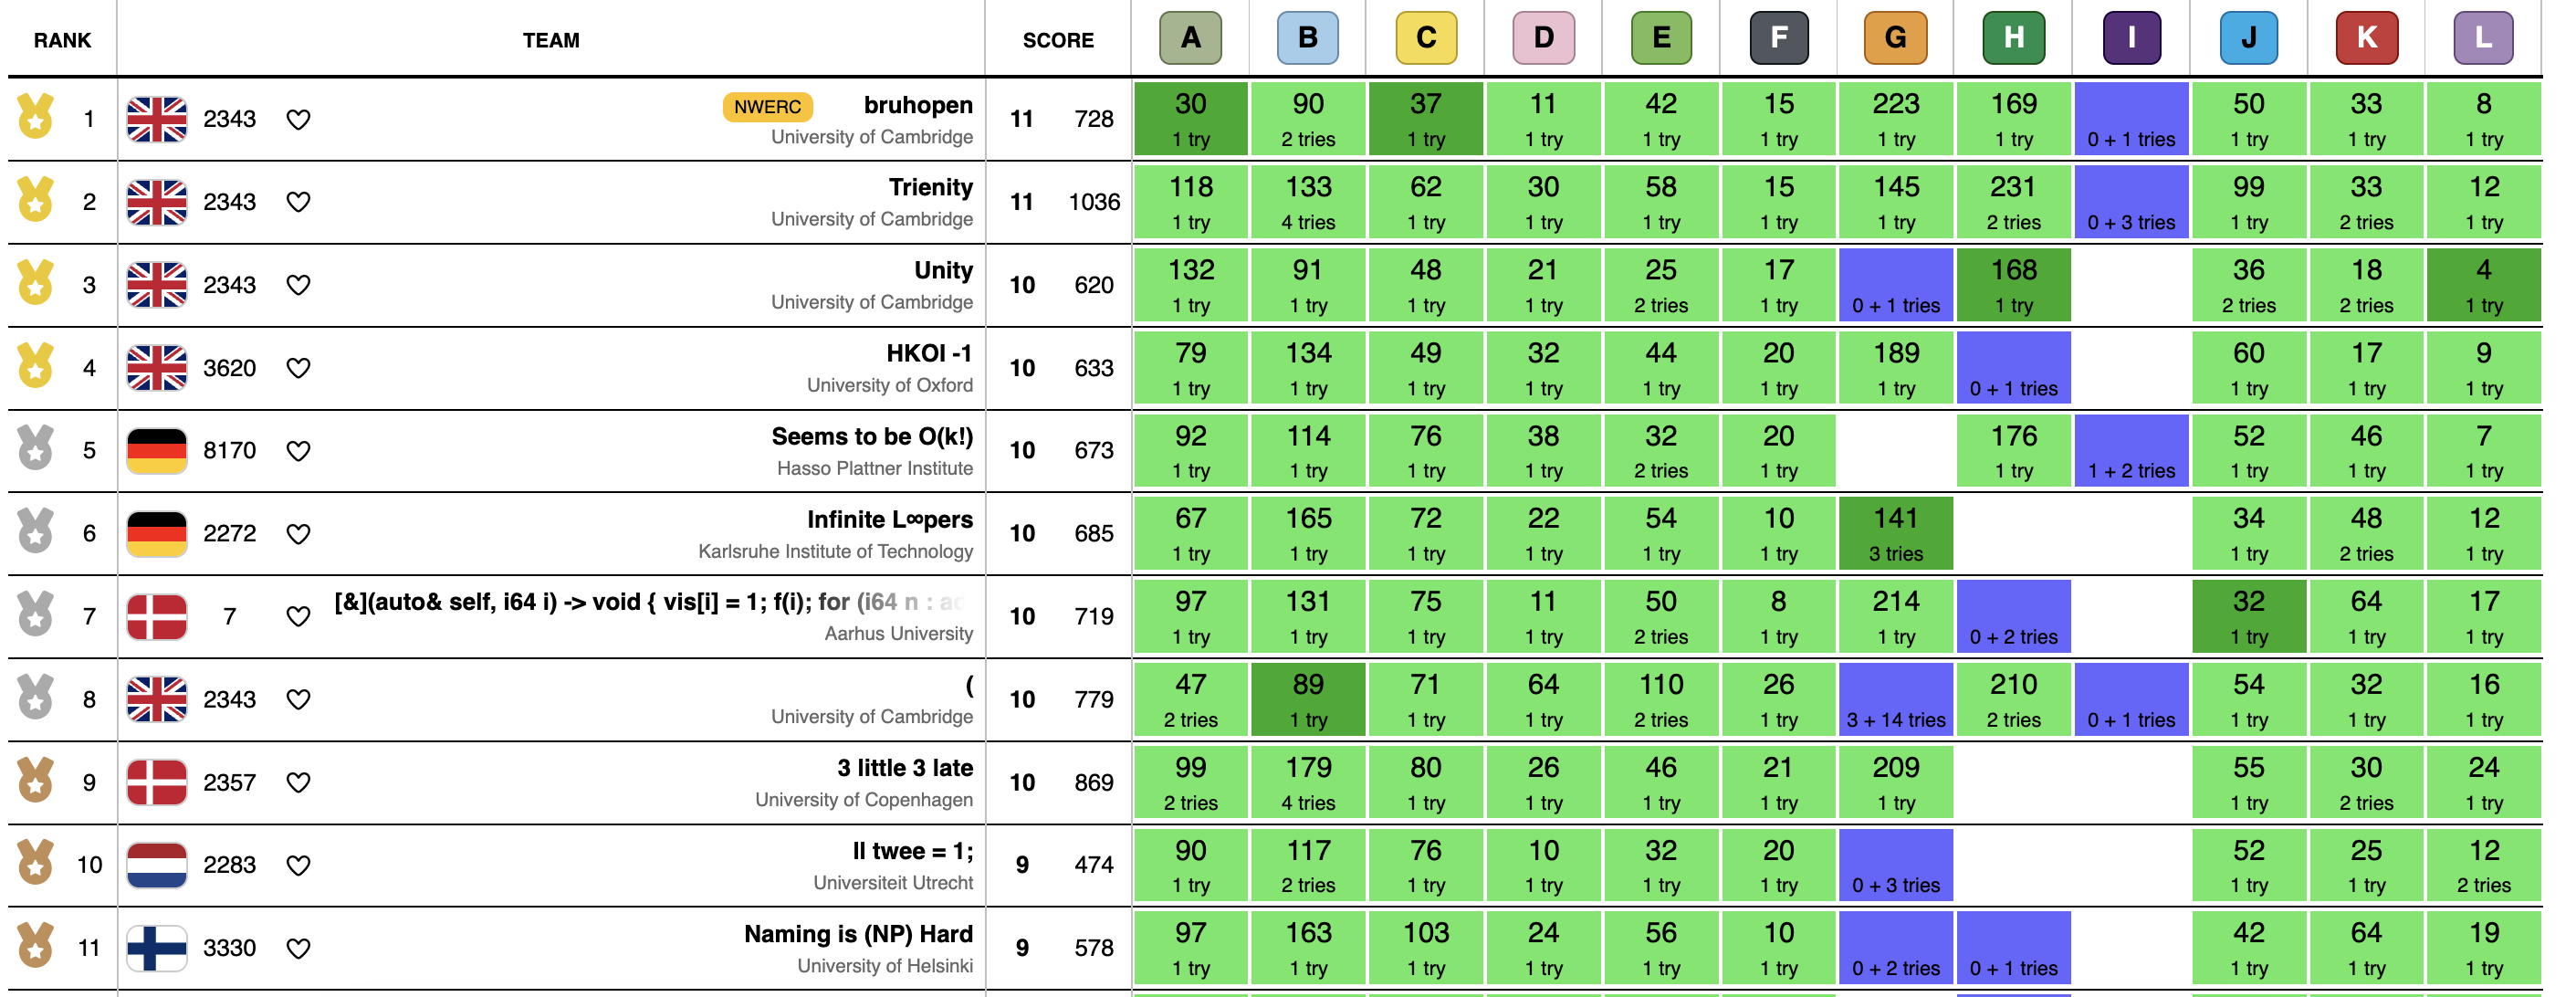
\includegraphics[width=\textwidth]{Imagenes/Vectorial/juez2.png}
  \caption{Interfaz de administración de DOMjudge mostrando el panel de control del concurso, con el estado de los judgehosts y los envíos recientes.}
  \label{fig:juez2}
\end{figure}

Cuando un equipo envía una solución, el DOMserver encola el envío y lo asigna al primer judgehost disponible. El judgehost descarga el código fuente, lo compila con el compilador correspondiente al lenguaje elegido y lo ejecuta contra cada caso de prueba dentro de un entorno de aislamiento que impide el acceso a la red, limita el tiempo de CPU y restringe el uso de memoria mediante \textit{cgroups}. El veredicto resultante es devuelto al DOMserver, que lo registra en la base de datos, actualiza el marcador y genera un evento en el feed de la API, haciéndolo inmediatamente disponible para cualquier sistema externo conectado, incluido el plugin de RA de este TFG.

\subsection{API REST de DOMjudge}
\label{subsec:domjudge_api}

La funcionalidad más relevante para este trabajo es la \textbf{API REST} de DOMjudge, que expone en formato JSON el estado completo del concurso de forma pública y sin interferir en su funcionamiento. A través de esta interfaz es posible consultar en tiempo real toda la información necesaria para construir la visualización de RA sobre la retransmisión: el marcador actualizado, los veredictos de los envíos, los datos de los equipos y el estado general del concurso.

\subsubsection*{Especificación Contest API}

DOMjudge implementa la \textbf{Contest API Specification} desarrollada por ICPC Tools, un estándar abierto diseñado para garantizar la interoperabilidad entre el sistema de jurado y herramientas externas de análisis, visualización y retransmisión. Esta especificación define los formatos de respuesta, los endpoints disponibles y el mecanismo de \textit{event feed} para la comunicación en tiempo real. La API es accesible en la ruta base \texttt{/api/v4/} del servidor DOMjudge. La mayoría de los endpoints de consulta son públicos y no requieren autenticación; únicamente las operaciones de escritura (envío de soluciones, configuración del concurso) requieren credenciales.

\subsubsection*{Endpoints principales}

La tabla~\ref{tab:domjudge-endpoints} recoge los endpoints más relevantes para la integración con el plugin de RA, con su método HTTP y una descripción de la información que proporcionan.

\begin{table}[H]
\centering
\small
\begin{tabularx}{\textwidth}{l l X}
\toprule
\textbf{Método} & \textbf{Endpoint} & \textbf{Descripción} \\
\midrule
GET & \texttt{/contests} & Lista todos los concursos disponibles, con identificador, nombre y estado. \\[4pt]
GET & \texttt{/contests/\{cid\}/scoreboard} & Marcador completo: posición, problemas resueltos, intentos y penalización de cada equipo. \\[4pt]
GET & \texttt{/contests/\{cid\}/submissions} & Lista de envíos: equipo, problema, lenguaje y marca de tiempo. \\[4pt]
GET & \texttt{/contests/\{cid\}/judgements} & Veredictos asociados a cada envío (AC, WA, TLE, etc.). \\[4pt]
GET & \texttt{/contests/\{cid\}/teams} & Equipos participantes: nombre, institución, país y metadatos. \\[4pt]
GET & \texttt{/contests/\{cid\}/problems} & Problemas del concurso: nombre, color del globo, límites de tiempo y memoria. \\[4pt]
GET & \texttt{/contests/\{cid\}/organizations} & Instituciones participantes con nombre y país, útil para mostrar logos o banderas. \\[4pt]
GET & \texttt{/contests/\{cid\}/event-feed} & Feed de eventos en tiempo real (Server-Sent Events): secuencia continua de cambios en el concurso. \\
\bottomrule
\end{tabularx}
\caption{Principales endpoints de la API REST de DOMjudge relevantes para la integración con el plugin de RA.}
\label{tab:domjudge-endpoints}
\end{table}

\subsubsection*{El event feed y los eventos en tiempo real}

El endpoint \texttt{/event-feed} es el mecanismo que permite al plugin de RA reaccionar a los eventos del concurso sin necesidad de hacer \textit{polling} periódico. Implementa el protocolo \textbf{Server-Sent Events (SSE)}: el cliente abre una conexión HTTP persistente y el servidor envía líneas de JSON conforme ocurren los eventos. En el instante en que un equipo recibe un veredicto \textit{Accepted}, el DOMserver genera un evento de tipo \texttt{judgements} y lo envía a todos los clientes conectados al feed. Cada evento tiene el siguiente formato:

\begin{verbatim}
{"id":"12345","type":"judgements","op":"create",
 "data":{"id":"j-42","submission_id":"s-17",
         "judgement_type_id":"AC",
         "start_time":"2025-03-15T10:32:44.712+01:00",
         "end_time":"2025-03-15T10:32:45.003+01:00"}}
\end{verbatim}

El campo \texttt{type} indica la entidad afectada (\texttt{submissions}, \texttt{judgements}, \texttt{teams}, etc.), \texttt{op} indica si es una creación o actualización, y \texttt{data} contiene el objeto completo. Cruzando el identificador del envío con los datos de equipos y problemas obtenidos mediante los endpoints correspondientes, el plugin puede construir el mensaje completo: qué equipo resolvió qué problema, cuándo, y cuál es su nueva posición en el marcador. Esta información es la que se superpone en tiempo real sobre la imagen de la cámara en la retransmisión.

\subsubsection*{Documentación interactiva e instancia de prueba pública}

DOMjudge proporciona una \textbf{documentación interactiva de la API} basada en OpenAPI (Swagger UI), accesible en la ruta \texttt{/api/doc} de cualquier instancia. Esta interfaz permite explorar todos los endpoints disponibles, consultar los esquemas de respuesta y realizar peticiones de prueba directamente desde el navegador.

Para el desarrollo y las pruebas del plugin de este TFG, DOMjudge ofrece una \textbf{instancia pública de demostración} permanentemente disponible en \url{https://www.domjudge.org/demoweb/}. Esta instancia contiene datos de un concurso ficticio con equipos, envíos y veredictos de ejemplo, y expone exactamente la misma API que un servidor real. El acceso es libre con las credenciales de ejemplo proporcionadas en la propia página. La documentación interactiva de esta instancia se encuentra en \url{https://www.domjudge.org/demoweb/api/doc}.

La integración con esta API es la que permite al plugin de OBS Studio consultar el marcador y los eventos del concurso en tiempo real, posibilitando superponer sobre la retransmisión información actualizada al instante: el equipo que acaba de resolver un problema, su posición en la clasificación o el tiempo transcurrido. Esta capacidad es la que conecta directamente el trabajo de este TFG con el dominio de los concursos de programación, trasladando al ámbito académico la misma experiencia de retransmisión enriquecida con RA que se aplica en eventos deportivos de gran escala como los descritos en el capítulo anterior.
\section{Conclusiones del Estado de la Cuestión en Concursos de
Programación}
\label{sec:conclusiones_concursos}
Una vez analizada la estructura operativa de los concursos de programación ylas herramientas que los sustentan, se han identificado los  pilares necesarios para dotar de inteligencia de datos al sistema de Realidad Aumentada propuesto en este TFG.

El estudio del formato ICPC ha revelado que la información crítica no reside
únicamente en el marcador final, sino en el flujo constante de eventos
(\textit{submissions}) y veredictos del juez automático. Para que la
Realidad Aumentada sea efectiva en una retransmisión, debe ser capaz de
reaccionar a estos eventos de forma síncrona. La investigación ha permitido
concluir que:
\begin{itemize}
\item \textbf{Relevancia del tiempo real}: El sistema debe priorizar la
visualización de los \textit{first solves} y los cambios de posición en el
\textit{rank}, ya que son los momentos de mayor impacto narrativo.
\item \textbf{Estandarización}: La dependencia de un sistema de gestión
de concursos (CMS) robusto es indispensable. La arquitectura de DOMjudge se
presenta como la solución ideal por su amplia adopción y su cumplimiento de
los estándares internacionales de la comunidad competitiva.
\end{itemize}

La revisión de la API REST de DOMjudge ha sido determinante para definir la
arquitectura del plugin de OBS. Se utilizarán los endpoints
\texttt{/contests}, \texttt{/teams} y \texttt{/scoreboard} como fuentes
primarias. La capacidad de obtener respuestas en formato JSON facilita el
parseo directo dentro del entorno C++ del plugin, permitiendo una
actualización de los activos 3D sin interrumpir el flujo de vídeo.

Con el cierre de este capítulo, se completa la fase de investigación del
"Estado de la Cuestión". Se dispone ahora de un marco teórico doble: por un
lado, el conocimiento técnico sobre RA, visión por computador y renderizado 3D
en OBS~\ref{cap:estadoDeLaCuestion}, y por otro, la comprensión de la lógica y la extracción
de datos de los concursos de programación~\ref{cap:concursos_programacion}.
Esta base permite abordar con garantías el siguiente bloque del trabajo: la
\textbf{Descripción del Trabajo de Realidad Aumentada}~\ref{cap:descripcionTrabajo}. En dicho capítulo se
detallará el proyerto detallado de la integración de RA en elmundo de OBS. Yposteriormente cómo se fusionan finalmente los datos del marcador de DOMjudge con la estimación de pose de OpenCV para generar la experiencia de visualización
enriquecida que motiva este proyecto \ref{cap:descripcionTrabajoConcursosProgramacion}.
